\chapter{Проектирование модели поведения виртуального агента}

В этом разделе описывается и обосновывается выбор инструментария для проектирования и программного воплощения 
модели поведения актора в заданной парадигме. Описываются ключевые моменты проектирования и программной реализации модели поведения актора.

\section{Проектирование модифицированного прототипа Виртуального Актора}

В данном разделе описывается реализация когнитивной модели в виде функций, интерпретируемых в форме псевдокода. Здесь приведены основные функции, вызываемые при работе алгоритма по выбору действия для Виртуального Агента. В начале будет описан алгоритм по выбору ответного действия Виртуального Актора на действие человека. 

На вход поступает действие человека, целью которого является влияние на Виртуального Актора. В зависимости от характеристики действия пересчитываются оценки Appraisals человека и Виртуального Актора по формуле 3. Соответственно уже на данном этапе меняется характеристика взаимодействующих акторов, что может повлиять на выбор ответного действия пингвина. Следующим шагом в соответствии с режимом работы моральной схемы производится вычисление новых значений векторов Feelings для взаимодействующих акторов.

Работа моральной схемы, следующая - по умолчанию она выключена и значения Feelings вычисляются по формуле 4. В этот момент времени моральная схема не оказывает никакого воздействия на принятие решения Виртуальным Актором. При отклонении абсолютного значения вектора Feelings от начального положения больше, чем на заранее заданную константу StartMoralSchema - моральная схема начинает свою работу. Ее функционирование происходит теперь в двух режимах:
\begin{enumerate}
  \item Feelings вычисляется по формуле номер 5 в случае, если  (расхождение между Feelings и Appraisals больше заранее определенной константы). Данный режим работы моральной схемы называется конфликтным. В таком ключе продолжается работа пока верна формула, описанная выше.
  \item Feelings константна и экстремальна по своим параметрам. Это означает, что Виртуальный Актор понимает каким образом нужно относиться к человеку: как к другу или врагу, как к подчиненному или начальнику и т.д. В данном режиме схема работает до тех пор, пока расхождения между Feelings и Appraisals не станет критическим. В этом случае снова включается режим номер 1.
\end{enumerate}

Возможен также вариант, когда отклонение Feelings от начального положения крайне мало. В таком случае моральная схема снова выключается и Feelings вычисляется по формуле 4. 

Первая функция описывает работу моральной схемы. В данной функции определяется режим работы моральной схемы и каким образом будет меняться субъективная оценка человека в отношении Виртуального актора.

На данном этапе получается следующая картина - обработано действия человека, направленное на пингвина, и пересчитаны “оценки” и “чувства” взаимодействующих акторов. Далее на основе соматического критерия и когнитивного фактора вычисляются вероятности для всех возможных действий в данной ситуации. Набор всех действий для Виртуального Актора заранее описан в *. json файле и у каждого действия есть параметр, который определяет в каком контексте оно применимо. Соответственно после определения действий применимых в данной ситуации, для каждого из них вычисляется вероятность на основе когнитивного фактора по формуле 6, на основе соматического по формуле 7 и итоговая вероятность по формуле 8. 

Следующим шагом необходимо определить ответное действия для пингвина из возможных с использованием ранее посчитанных для них вероятностей. Все действия сортируются по возрастанию численного значения их вероятностей. При помощи функции рандомной генерации чисел, основанной на равномерном распределении, генерируется дробное число от 0 до 1. Далее по формуле 9 определяется ответное действие.

Где  - вероятность i-го действия, k - число, пробегающее от 1 до n, где n - общее количество рассматриваемых действия для Виртуального Агента. Минимальное k, при котором выполняется неравенство, описанное в формуле 9, соответствует номеру действия в списке действий, отсортированном по возрастанию вероятностей. Это действие и будет совершено Виртуальным Актором.

Предпоследним этапом работы алгоритма является пересчет значений Appraisals и Feelings по описанной в начале данного пункта схеме.

В конце действие, которое должен выполнить пингвин возвращается в виде строкового значение в функцию, отвечающую за перемещение и действия пингвина в виртуальном окружении и выбранное действие визуализируется Виртуальным Актором. После этого человек может снова совершить воздействие на пингвина, и вся данная процедура снова повторится. 

Далее будет описан алгоритм выбора самостоятельного действия Виртуальным Актором. Под самостоятельным действием понимается такой действия, которое предпринимает пингвин, основываясь на состоянии виртуального окружения и отношении с человеком. Алгоритм выбора самостоятельного действия схож с алгоритмом выбора ответного действия на действие со стороны человека, направленное на Виртуального актора. Исполнение начинается с шага вычисления вероятностей для возможных в данной ситуации действий на основе когнитивного и соматического фактора. В данной парадигме возможно проявление одного из следующих взаимодействий со стороны пингвина:

\begin{itemize}
  \item Подойти к корзине со снежками с желанием поиграть
  \item Подойти к корзине с рыбой и попросить поесть
  \item Подойти к человеку с целью взаимодействия с ним
  \item Пойти спать
  \item Посмотреть в сторону человека
  \item Поприветствовать человека
\end{itemize}
  
Здесь может быть проблема с бесконечной очередью вызовов действий без временного интервала между ними. Тогда взаимодействие с Виртуальным агентом может стать проблематичным. Возможны два пути решения данной проблемы. Первое решение — это создание некоторого минимального промежутка времени после выполнения самостоятельного действия пингвина, в течение которого, программно будет запрещено совершение самостоятельного действия для Виртуального Актора. Такой подход в определенной мере решает проблему бесконечной непрерывной очереди действий пингвина, однако он довольно искусственный и слабо согласуется с моделью социально-эмоционального интеллекта на основе когнитивной архитектуры eBICA. Второй подход заключается в создании действий “заглушек”, которые практически не влияют на соматические и когнитивные оценки акторов. Данными действиями могут быть, например:
\begin{itemize}
\item Пингвин стоит на месте
\item Пингвин перемещается по виртуальному окружению в какую-либо его точку
\end{itemize}

При совершении этих действий оценки Виртуального Актора и человека практически не будут меняться и будет создан временной интервал между социальными действиями пингвина. 

% \section{Адаптация модели поведения виртуального агента}
% тут вообще можно нахуярить во второй клаве из статьи про акустические признаки
% с одним или двумя слоями по 80 нейронов в каждом и выходом в восьминейронный слой.
% *** картинка Figure 2. Proposed pipelines for speech emotion recognition. из файла в телеге applsci-12-00327.pdf *** В иделе на ру перевести и расширить главу
\section{Инструменты извлечения речевых признаков из речи}

В связи с задачей эмоционального взаимодействия пользователя с вирутальным актором
ставится задача распознавания эмоциональной составляющей из человеческой речи. А также
классификация эмоционального воздействия.

Так как в данной работе для анализа человеческой речи используется нейросеть, а это значит,
что требуется дата-сет для обучения данной нейросети.
В большинстве работ по классификации эмоций присутствующих в речи человека используются
открытые данные RAVDESS. Этот дата-сет включает в себя 7356 аудио записей с эмоциональным наполнением.

Область распознавания речи и ее эмоциональной составляющей довольно обширна. И решение данной задачи с нуля
является слишком трудозатратной. Поэтому в работе будет использована предобученная модель.
Данная модель позволит преобразовывать аудиоинформацию в векторное пространство.

Вектор полученный из записи человеческой речи будет использован для обучения нейронной сети,
которая по признакам вектора определит эмоциональную составляющую.

Для того, чтобы получить решение данной задачи будут использованы такие модели (Рис. \ref{pic:normpic}):

\begin{figure}[h]
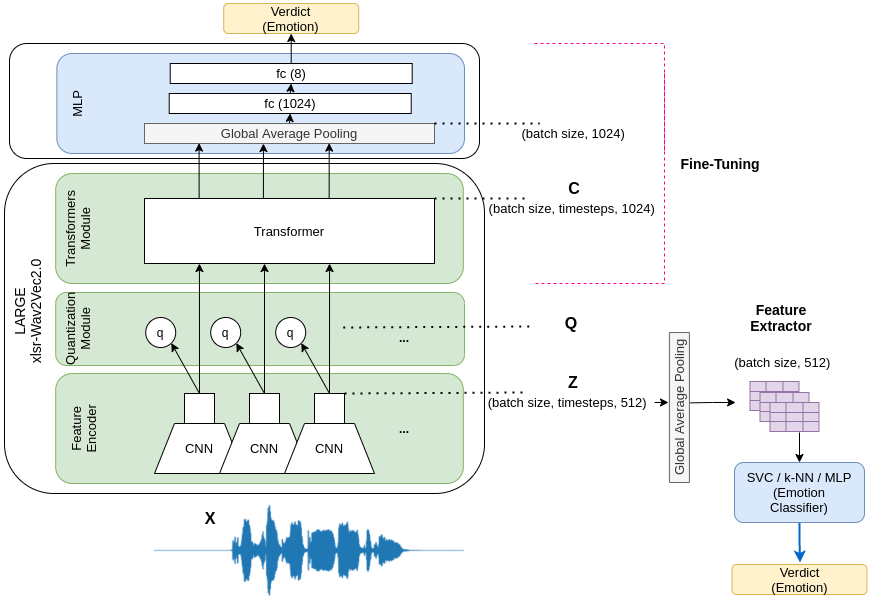
\includegraphics[width=0.75\columnwidth]{./img/normpic.png}
\centering
\caption{Предлагаемые конвейеры для распознавания речевых эмоций.}
\label{pic:normpic}
\end{figure}


SVM с ядром «RBF» -  является одной из наиболее популярных методологий обучения по прецедентам,
предложенной В. Н. Вапником и известной в англоязычной литературе под названием SVM (Support Vector Machine).

k-ближайших соседей (kNN) с большинством голосов для выбора класса - 
расшифровывается как k Nearest Neighbor или k Ближайших Соседей — это один из самых простых алгоритмов классификации, также иногда используемый в задачах регрессии. 

Многослойный персептрон (MLP) -  это класс искусственных нейронных сетей прямого распространения, состоящих как минимум из трех слоёв: входного, скрытого и выходного.
За исключением входных, все нейроны использует нелинейную функцию активации.

% можно во второй главе чото о психологах насрать
% \section{Модель определения эмотивной составляющей в тексте}

% Текст человеческой речи позволяет передать не только непосредственно смысл, который закладывает в нее говорящий,
% но и эмоциональную составляющую. Конечно текстовый формат представления не позволяет передать интонацию, но
% даже по тексту можно выявить эмоцию говорящего.

% В данной работе требуется в дополнение к эмоциональной оценке по аудиозаписи получить эмоциональную оценку
% по тексту. Что позволит наиболее точно установить эмоциональное взаимодействие с виртуальным актором.
% Так же такой анализ позволит выявить случаи сарказма в речи пользователя.

% В современных системах автоматического определения эмоциональной
% оценки текста чаще всего используется одномерное эмотивное пространство:
% позитив-негатив, то есть хорошо-плохо.

% Поэтому для упрощения будем классифицировать тексты по шкале:

% \begin{enumerate}
%   \item негативная оценка
%   \item позитивная оценка
% \end{enumerate}

% Автоматическое определение тональности текста подразумевает выделение тех фрагментов текста, 
% которые выражают позитивную или негативную эмоциональность по отношению к объекту эмоциональной оценки (объекту
% тональности). Объект эмоциональной оценки может быть задан как один
% в целом для текста (с учетом его синонимических и анафорических употреблений), 
% так и определяться в предложениях как любое имя собственное или даже нарицательное.

% Сегодня уже существуют достаточно точные решения, определяющие эмоциональную составляющую текста.
% Но большинство таких решений являются нейросетями обученными на полноценных текстах редко включающих в себя
% диалоговую составляющую. Тогда как в работе требуется только анализ диалогов. Поэтому
% будет взята модель анализа тональности текста c использованием правил объединения слов в цепочки
% и определения тональности у объекта на основе предикационных отношений
% в пропозиции и дообучена на диалоговых данных, которые 
% будут собраны посредством фильтрации диалогов из публично доступных дата-сетов с сохранением разметки.

% %\section{Инструменты для анализа текста}
% % тут чисто про w2vec то есть получение конкретных команд пингвином
\section{Инструменты для семантического анализа текста}

После того как речь была распознана и конвертирована в текстовый формат ставится задача определить
семантической смысл предложения.  

Возможность идентификации семантической близости между словами сделала модель word2vec широко используемой в NLP-задачах, которые подробно описываются в \cite{neural05}. 
Идея word2vec основана на контекстной близости слов. Каждое слово может быть представлено в виде вектора, 
близкие координаты векторов могут быть интерпретированы как близкие по смыслу слова \cite{seman04}. 

Таким образом, извлечение семантических отношений (отношение синонимии, родовидовые отношения и другие) может быть автоматизировано. 
Установление семантических отношений вручную считается трудоемкой и необъективной задачей, требующей большого количества времени и 
привлечения экспертов. Но среди ассоциативных слов, сформированных с использованием модели word2vec, встречаются слова, не 
представляющие никаких отношений с главным словом, для которого был представлен ассоциативный ряд \cite{seman03}.

В работе рассматриваются дополнительные критерии, которые могут быть применимы для решения данной проблемы. Наблюдения и проведенные 
эксперименты с общеизвестными характеристиками, такими как частота слов, позиция в ассоциативном ряду, могут быть использованы для 
улучшения результатов при работе с векторным представлением слов в части определения семантических отношений для русского языка. 

Представление слов в виде векторов позволяет применять математические операции. В большинстве примеров можно встретить вычитание векторов, 
когда результат вычисления vec('Таллин') - vec('Эстония') + vec('Россия') будет ближе к vec('Москва'), чем к другим векторам из распределения. 
Таким образом, разница векторов может быть использована для поиска семантических отношений между словами \cite{seman02}.

Word2vec не возвращает напрямую семантические отношения между словами. В ассоциативном ряду, который может быть возвращен 
в качестве близких слов к запрашиваемому (главному) слову, отражаются слова, которые часто употребляются рядом в контексте. 
Бесспорно, в ассоциативном ряду встречаются синонимы, антонимы, гипонимы, гиперонимы, холонимы, меронимы, ассоциации и другие 
типы, которые могут быть определены как семантические отношения.


Для реализации используются такие пакеты языка программирования python как: ufal.udpipe и wget. 
Как было сказано ранее для нахождения близости слов мы используем готовую модель, которую взяли с ресурса 
https://rusvectores.org/static/models с помощью пакета wget, принцип работы описан в \cite{neural08}. Данный пакет позволяет скачивать данные 
с веб ресурсов посредством GET запроса.

Для того чтобы модель word2vec, описанная в \cite{w2vec02} могла определить расстояние между словами, ей следует передать слово, ставится задача определить 
его часть речи, для того, чтобы автоматизировать такой процесс по определению части речи слова из текста, мы должны с помощью 
системы word2vec понять по слову какими категориями частей речи оно обладает, самые распространённые варианты – это 
существительные и глагол, далее после определения,  мы передаем их на анализ дистанции. 
Принцип работы модели представлен на (Рис. \ref{pic:ris15}):

\begin{figure}[H]
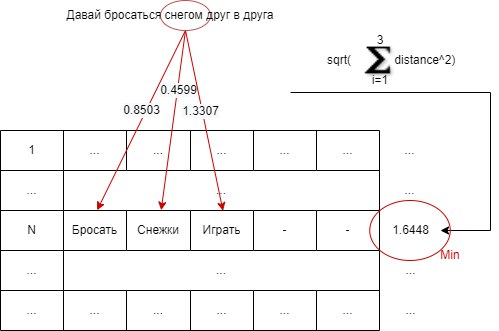
\includegraphics[width=0.75\columnwidth]{./img/ris15.png}
\centering
\caption{принцип работы word2vec}
\label{pic:ris15}
\end{figure}

В рамках данной работы используется модель ruwikiruscorpora\_tokens\_elmo\_1024\_2019 - модель UDPipe для нахождения синонимов. 
Данная модель позволяет узнать семантическую близость слов.

Чтобы начать применять указанную выше нейронную сеть непосредственно, следует подготовить действия виртуальных акторов так, 
чтобы ими могла оперировать частично или полностью сама нейронная сеть. Для этого возьмем разобьем описание каждого действия 
на ключевые слова так, что каждое действие будет ассоциировано с набором слов. При этом создан класс отражающий действие 
актора как сущность - VAAction(Virtual Actor Action), принцип которой описан в \cite{w2vec01}.

Данный класс содержит в себе описание действия и ключевые слова, описывающие данное действие. 
Среди таких слов отсутствуют предлоги, а сами слова представлены в нормальной форме 
(для существительных - именительный падеж единственное число).

Для построения сценариев берутся текста, полученные в разделе выше. Для каждого текста выделяются ключевые слова, 
которые наиболее близки к ключевым словам, описывающим действия акторов. Что происходит в процессе итерации через 
все слова текста так, что для каждого слова применяется считается значение близости слова к действию виртуального 
актора. Для работы с текстом создан класс WText (Web Text), который является ответственным за итерацию через все 
слова текста. С помощью методов класса задается функция, которая будет применяться к каждому слову. В качестве 
такой функции берется функция, которая находит близость слова с ключевыми словами экземпляра класса VAAction.

Также класс WText формирует набор определяющих текст слов, эти слова выбираются так, что значение 
семантической близости больше, чем заданный заранее порог, данной работе порог равен 0.08. После 
того как все тексты были переведены в экземпляры класса WText, была произведена оценка кол-ва 
текстов с одинаковым кол-вом определяющих слов.

\section{Построение блок-схем и UML диаграмм}

В данном разделе строятся блок-схемы реализованного алгоритма (Построение такой диаграммы рекомендуется в работе \cite{OOP}).
На (Рис. \ref{pic:oldcmodel0}) представлена упрощенная блок-схема работы алгоритма по выбору ответного действия для актора.
Данный алгоритм срабатывает каждый раз после совершения действия человеком, которое направлено на пингвина.
Также данный алгоритм может приостанавливать любое продолжительное действие самого пингвина. 

\begin{figure}[h]
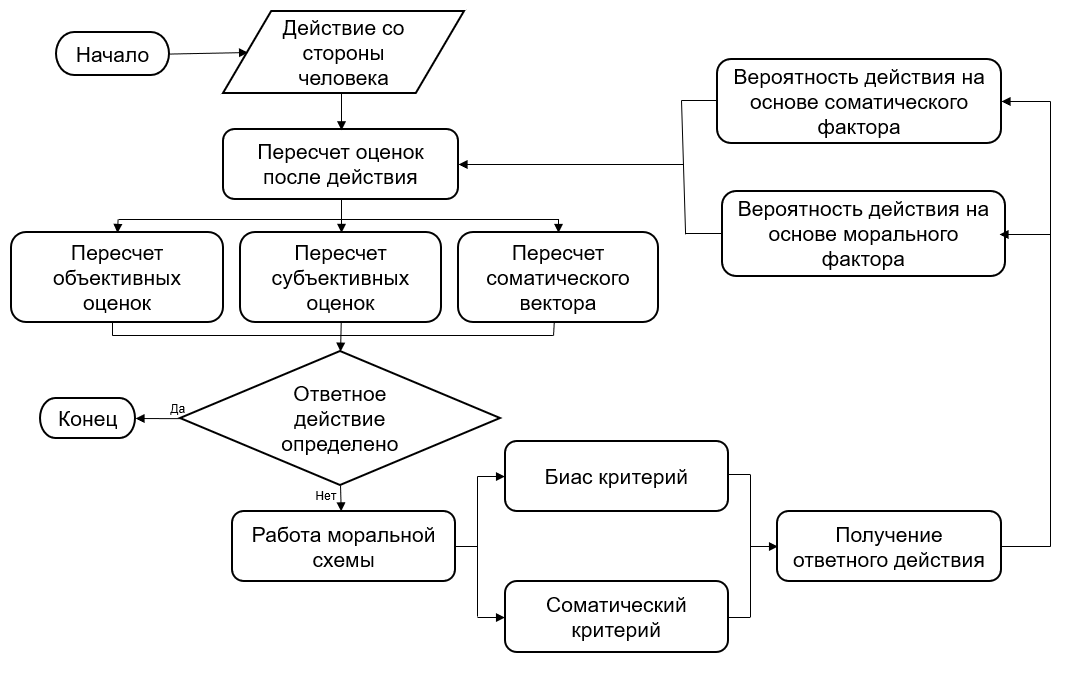
\includegraphics[width=0.75\columnwidth]{./img/oldcmodel0.png}
\centering
\caption{Блок-схема общей работы алгоритма}
\label{pic:oldcmodel0}
\end{figure}

На вход поступает действие человека, направленное на пингвина. На основе оценок данного действия пересчитывается Appraisals и Feelings человека и пингвина, а также 
вектор соматического состояния. Затем последовательно срабатывают две функции: Критерий Биас и Соматический критерий. 
В них определяется вероятность для каждого действия на основе когнитивного и соматического состояния соответственно.
Далее на основе данных вероятностей определяется итоговое действие, которое будет выполнено пингвином. 
Данное действие определяется наибольшей вероятностью. 

Рассмотрим более подробно алгоритм пересчета Feelings (субъективных оценок) для акторов. На (Рис. \ref{pic:oldcmodel1}) представлена блок-схема данного алгоритма. На вход поступают Appraisals и Feelings актора. 
Затем, если до этого никогда данному актору не присваивалась константная оценка Feelings, то Feelings присваивается значение согласно уравнению, 
когда моральная схема выключена и не оказывает никакого воздействия на вектор Feelings. 
Если Feelings актора уже принимал заданное константное экстремальное значение, то Feelings присваивается значение в зависимости от разницы норм Feelings и Appraisals.

\begin{figure}[h]
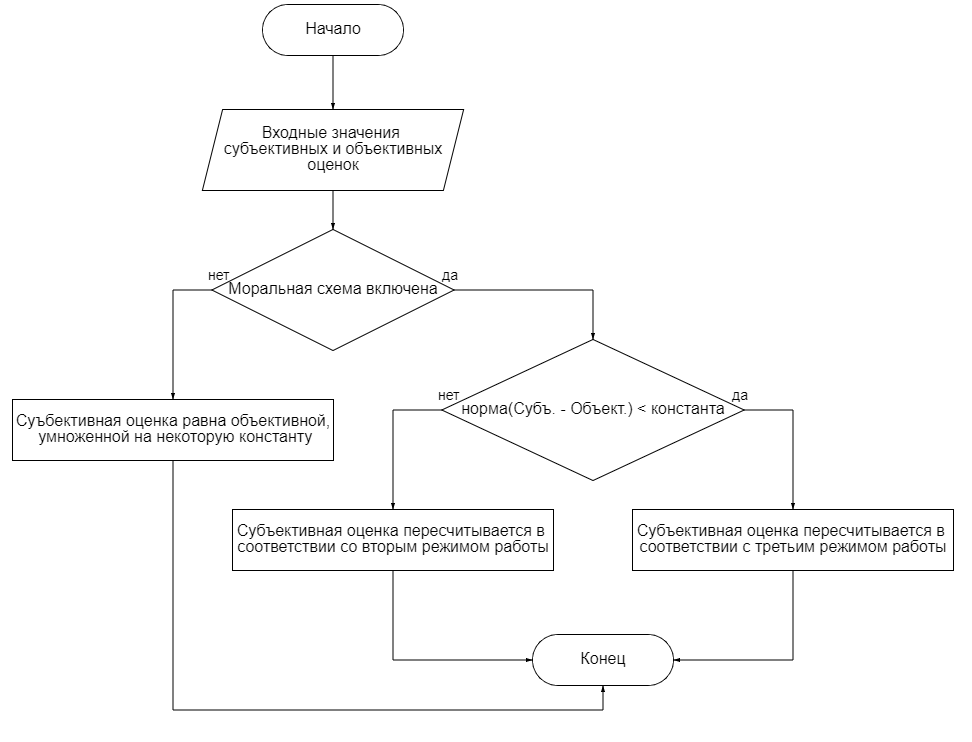
\includegraphics[width=0.75\columnwidth]{./img/oldcmodel1.png}
\centering
\caption{Блок-схема алгоритма пересчета значений Feelings акторов}
\label{pic:oldcmodel1}
\end{figure}

На (Рис. \ref{pic:oldcmodel2}) показана диаграмма классов, описывающая процедуру взаимодействия Виртуального Агента и человека. 
Диаграмма наглядно демонстрирует взаимосвязь человека и 
Виртуального Актора с методами логирования и выбора действий для пингвина с пересчетом “оценок” и “чувств”. 
При использовании данной схемы алгоритм поведения Виртуального Актора, основанного на когнитивной архитектуре eBICA, можно легко перенести и адаптировать 
под другую парадигму и виртуальное окружение.

\begin{figure}[h]
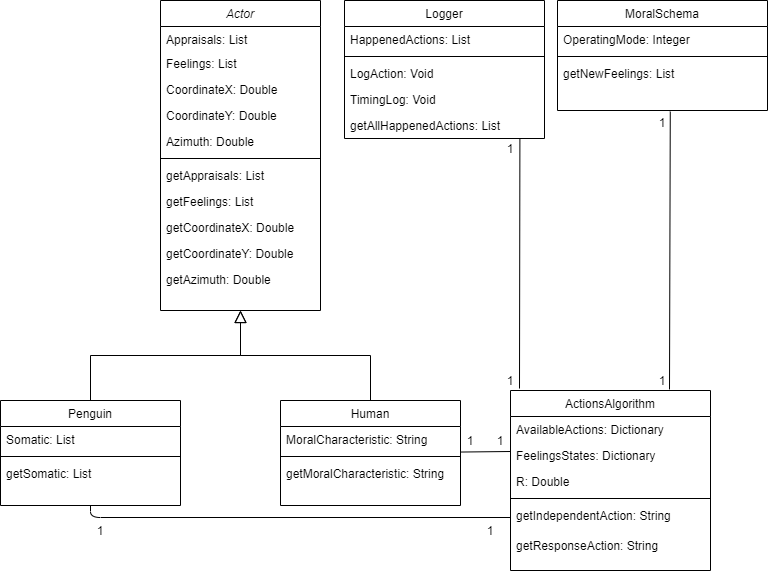
\includegraphics[width=0.75\columnwidth]{./img/oldcmodel2.png}
\centering
\caption{Диаграмма классов, описывающая взаимодействие Виртуального агента и человека}
\label{pic:oldcmodel2}
\end{figure}


Класс Human описывает характеристики человека, проводящего игровую сессию с пингвином. 
Класс Penguin представляет собой Виртуального Агента, реализованного в виде пингвина в виртуальном окружении. 
Human и Penguin наследуются от общего класса Actor и имеют характеристики: Appraisals - “оценки”, Feelings - “чувства”, 
CoordinateX, CoordinateY, Azimuth - координаты местонахождения в виртуальном окружении и угол поворота относительно севера (
север представляет собой сильно удаленную точку от площадки взаимодействия человека и пингвина и определен заранее).  
Также у классов Penguin и Human есть уникальные поля. У Penguin поле Somatic, которое представляет собой вектор соматического состояния, 
представленного структурой List. У Human поле MoralCharacteristic - представляет собой строковое значение, которое показывает, 
как пингвин относится к человеку с точки зрения моральной схемы. Penguin связан ассоциацией с классом ActionsAlgorithm. 
Данный класс отвечает за выбор действий для Виртуального Актора и обрабатывает действия человека. ActionsAlgorithm связан с классом MoralSchema, 
который представляет собой моральную схему. Принцип ее работы был описан в разделе 3.1. MoralSchema связана ассоциацией с Logger. 
Этот класс отвечает за логирование всех действий со стороны человека и пингвина. Также срабатывает функция TimingLog каждые 4 
секунды для сохранения в файл текущего состояния виртуального окружения.

В дополнение к классам приложения до модернизации проектируются классы для работы с человеческой речью (Рис. \ref{pic:ncmodel0}):

\begin{figure}[!h]
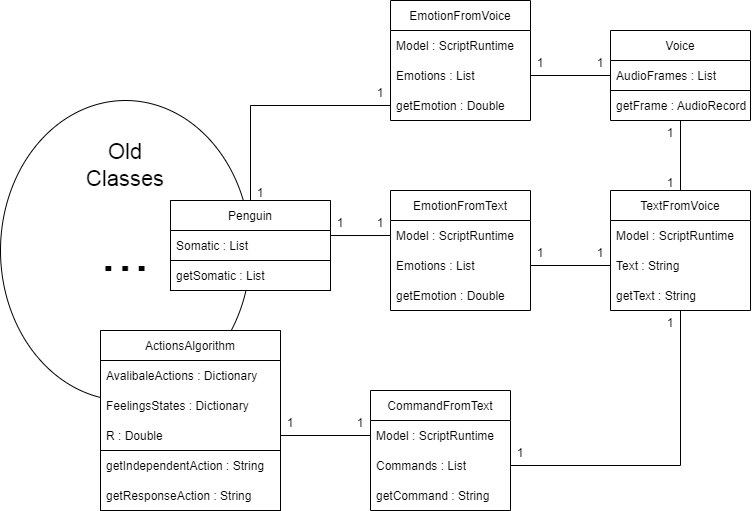
\includegraphics[width=0.75\columnwidth]{./img/ncmodel0.jpg}
\centering
\caption{Расширенная диаграмма классов с участием голосового распозвавания}
\label{pic:ncmodel0}
\end{figure}

Для работы с человеческой речью непосредственно используется класс Voice, который отвечает за фильтрацию речи и разбиение аудиодорожки на фреймы. 
Фреймы передаются в классы EmotionFromVoice   
и TextFromVoice. Первый извлекает эмоциональную составляющую из фрейма. Второй распознает речь   
и возвращает текст, который используется в классах EmotionFromText и CommandFromText.   
EmotionFromText как и EmotionFromVoice извлекает эмоциональную составляющую, но уже из текста. 
CommandFromText итерируется по полученному тексту и сопоставляет ключевые слова с действиями пи  
нгвина по алгоритму из рисунка \ref{pic:ris15} . Полученные команды передаются в   
ActionAlgorithm для того, чтобы увеличить вероятность выполнения распознанных действий. Все эмо  
циональные оценки передаются в Penguin и меняют его состояние соответсвующе.

Общая блок-схема работы алгоритма по анализу речи представлена на рисунке \ref{pic:block_schema}: 

\begin{figure}[!h]
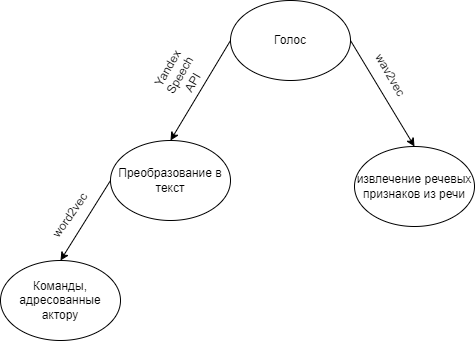
\includegraphics[width=0.75\columnwidth]{./img/block_schema.png}
\centering
\caption{Расширенная диаграмма классов с участием голосового распозвавания}
\label{pic:block_schema}
\end{figure}

На вход поступает аудио, которое анализуется 2мя способами, первое из которых преобразование текста в речь и 
анализ команды адресованной виртуальному питомцу. Второй из них определяет акустически эмоциональную окраску речи.
%Анализ команды адресованной ваиртуальному агенту

\section{Выводы}

Производилось проектирование модифицированного прототипа виртуального актора 
с учетом всех ключевых особенностей парадигмы объектно ориентированного программирования. 
Были разработаны модели семантического, эмоционального анализа речи.
